\chapter{Zona de estudio.}
\label{chap_zonaEstudio}

La zona de estudio se encuentra localizada en las afueras del per\'imetro urbano del municipio de Ciudad Bol\'ivar en el Departamento de Antioquia. 
Las laderas noroxidental y suroriental de la quebrada La Linda poseen pendientes que oscilan entre el \(20\,\%\) y \(30\,\%\)
% Es importante colocar el valor del área de la ladera.
La Quebrada La Linda no posee afluente alguno, sus aguas desembocan en su totalidad en la quebrada La Raya.
Las pendientes m\'as pronunciadas de la cuenca hidrogr\'afica de la quebrada La Linda se encuentran aguas arribas en las cercan\'ias del Batolito Farallones, tal como se puede apreciar en la Figura \ref{fig:slopes}.

\begin{figure}[H]
\centering
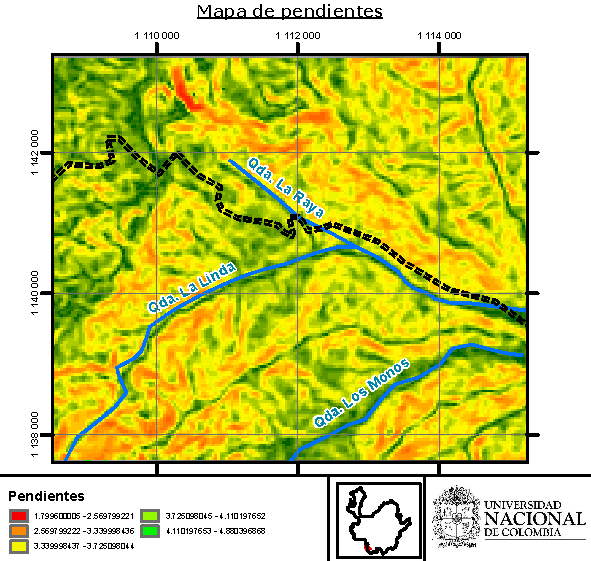
\includegraphics[scale=1]{img/pendientes.pdf}
\caption{Mapa de pendientes de la cuenca hidrogr\'afica de la quebrada La Linda y sus zonas circundantes. Elaboraci\'on propia}
\label{fig:slopes}
\end{figure}
La principal v\'ia de acceso es la carretera que desde el municipio de Ciudad B\'olivar conduce a El Carmen de Bol\'ivar.
